\section{Finite perturbations with divergent gain}\label{sec:tilts}

Fix a chart $I$, its slope $s>0$, and the partitions $\Pi_j$ from
Section~\ref{sec:budget}.  In this section suppose that, for some deterministic
$H_0\geq1$, the following event in an iid environment has probability $p>0$:
there is a bigeodesic through $0$ whose upper label belongs to $I$, avoids
all partition endpoints, and whose two arms lie in $Q^\pm(0,H_0)$.
Denote this event by $\mathcal B(0)$, and its horizontal translate to
$k=(k_1,0)$ by $\mathcal B(k)$.  The chart, $s$, $H_0$, and $p$ remain fixed
throughout the construction.  The eventual proof of \Cref{thm:main} will
reduce a positive probability of bigeodesics to precisely this situation.

We shall obtain, for every positive integer $M$, marks of probability
bounded below independently of $M$.  A mark comes with a bigeodesic in a
finite upward perturbation of the iid environment and a gain of at least
$M$ on an initial portion of that bigeodesic.  A second requirement, a
strictly raised edge within a fixed number $R_0$ of steps, will prevent
two marks on a suitably spaced horizontal grid from having the same
label.  The distinction between this fixed $R_0$ and the larger radius
needed for the gain $M$ is essential.

\subsection{A shared family of finite perturbations}

Bates and Chatterjee~\cite[Lemmas~2.3--2.4]{BatesChatterjee2020}
bound the change of product law for small Bernoulli replacements whose
distributions have bounded density relative to the original law.
The low-to-high replacement below is a monotone instance of this
construction; related spatially varying passage-time perturbations
appear in \cite[Section~2.3]{DembinElboimPeled}.
We derive its estimates directly, share the edge samples between sites,
and compute the conditional law given an individual modified environment.

Use the thresholds $a_0<b_0$ of \Cref{lem:usable}, and write
\[
 p_a=G([0,a_0])>0,\qquad p_b=G([b_0,\infty))>0,
 \qquad g=b_0-a_0>0.
\]
Thus $q=G([0,b_0))$ satisfies $8\sqrt q<1$.  An edge is usable when its
weight is at least $b_0$. Write $\mu=G^{\mathcal E}$ for the iid law of
the base environment; probability $\PP$ below is taken on the enlarged
coupling. Take, independently for every edge $e$, a triple
$(X_e,U_e,Z_e)$, where
\[
 X_e\sim G,\qquad U_e\sim\operatorname{Unif}[0,1],\qquad
 Z_e\sim G(\,\cdot\mid[b_0,\infty)).
\]
The coordinates of each triple are independent, as are the triples at
different edges.  The base environment is $X=(X_e)_e$, with metric $T$.
All variants below use these same triples.

For an edge $e$ with endpoints $w,w'$, put
\[
 h(e)=\max\{|w_2|,|w'_2|\},\qquad
 \delta_h=\frac{\eta}{(h+2)\log(h+2)},\quad h\geq0,
\]
where $\eta>0$ will be chosen shortly, independently of $M$.  Require
$\delta_0\leq p_a/2$, and define
\begin{equation}\label{eq:shared-raise}
 \xi_e=\mathbf1\{X_e\leq a_0,\ U_e\leq\delta_{h(e)}/p_a\},
 \qquad
 \widehat X_e=
 \begin{cases}
 Z_e,&\xi_e=1,\\
 X_e,&\xi_e=0.
 \end{cases}
\end{equation}
In particular $\widehat X_e\geq X_e$, and
$\widehat X_e-X_e\geq g$ whenever $\xi_e=1$.

For a horizontal site $k=(k_1,0)$ and an integer $R\geq1$, define the
finite set of edges
\begin{equation}\label{eq:tilt-region}
 A_k(R)=\left\{e:\ h(e)\leq R,\quad
  \max_{w\text{ endpoint of }e}|w_1-k_1|
       \leq1+\frac{h(e)+H_0}{s}\right\}.
\end{equation}
Let $Y^{k,R}$ equal $\widehat X_e$ on $A_k(R)$ and $X_e$ elsewhere,
and denote its metric by $T^{k,R}$.  For two horizontal sites $k,y$,
let $Y^{k,y,R}$ instead use $\widehat X_e$ on
$A_k(R)\cup A_y(R)$, with metric $T^{k,y,R}$.  In an overlap there is
one use of the same sample $\widehat X_e$.  We never apply the replacement
operation twice to an edge.

The absolute height in \eqref{eq:tilt-region} accommodates excursions in
either vertical direction.  Indeed, if a bigeodesic through $k$ has its
arms in $Q^\pm(k,H_0)$, then every vertex $w$ of either arm satisfies
\begin{equation}\label{eq:whole-path-width}
 s|w_1-k_1|\leq |w_2|+H_0.
\end{equation}
For the upper arm this follows from
$s|w_1-k_1|\leq w_2+H_0$, and for the lower arm from
$s|w_1-k_1|\leq-w_2+H_0$.  Consequently every edge of this bigeodesic
with $h(e)\leq R$ belongs to $A_k(R)$.  In particular its first $R$
upper-arm edges belong to this set: the $j$th edge has $h(e)\leq j$.

\begin{lemma}[Uniform change of law]\label{lem:likelihood}
Every individual environment $Y^{k,R}$ and every union environment
$Y^{k,y,R}$ has law absolutely continuous with respect to $\mu$.
There is a finite constant $C$, depending only on $s,H_0,p_a,p_b$, such
that the density $L_{k,R}=d\mathcal L(Y^{k,R})/d\mu$ satisfies
\begin{equation}\label{eq:likelihood-bound}
 \EE_\mu L_{k,R}^2\leq\exp(C\eta^2),\qquad
 \|\mathcal L(Y^{k,R})-\mu\|_{\mathrm{TV}}
 \leq\tfrac12\sqrt{\exp(C\eta^2)-1}.
\end{equation}
The bounds are uniform in $k$ and $R$.
\end{lemma}

\begin{proof}
The law of $\widehat X_e$, for $h(e)=h$, has density relative to $G$
\begin{equation}\label{eq:one-edge-density}
 \lambda_h(t)=1-\frac{\delta_h}{p_a}\mathbf1_{[0,a_0]}(t)
                 +\frac{\delta_h}{p_b}\mathbf1_{[b_0,\infty)}(t).
\end{equation}
The two indicated sets are disjoint.  Direct integration gives
$\int\lambda_h\,dG=1$ and
\begin{align}
 \int\lambda_h^2\,dG
 &=p_a(1-\delta_h/p_a)^2
    +p_b(1+\delta_h/p_b)^2+1-p_a-p_b\notag\\
 &=1+(p_a^{-1}+p_b^{-1})\delta_h^2.
 \label{eq:one-edge-second-moment}
\end{align}
For any deterministic finite set of replaced edges, independence of the
triples makes the full density the product of these one-edge densities;
the exterior has its original iid law.  This proves absolute continuity
for both the individual and union environments.

To bound the product for an individual region, let $N_h$ count its edges
of height $h$.  At positive height $h$, horizontal edges lie in the two
rows of heights $h,-h$, and vertical edges lie in the two strips adjoining
those rows toward height zero.  Each row or strip contains at most
$2(1+(h+H_0)/s)+1$ admissible edges.  At height zero there is only one
horizontal row.  Thus, for example,
\[
 N_h\leq c_s(h+H_0+1),\qquad c_s=12+8/s.
\]
It follows from \eqref{eq:one-edge-second-moment} that
\begin{align*}
 \EE_\mu L_{k,R}^2
 &=\prod_{e\in A_k(R)}
       \bigl[1+(p_a^{-1}+p_b^{-1})\delta_{h(e)}^2\bigr]\\
 &\leq\exp\left\{
 c_s(p_a^{-1}+p_b^{-1})\eta^2
 \sum_{h=0}^{\infty}
 \frac{h+H_0+1}{(h+2)^2\log^2(h+2)}\right\}.
\end{align*}
The series is finite; its terms of leading order are
$1/(h\log^2h)$.  It defines the required constant $C$.
Finally, since $\EE_\mu L_{k,R}=1$, Cauchy--Schwarz gives
\[
 \|\mathcal L(Y^{k,R})-\mu\|_{\mathrm{TV}}
 =\tfrac12\EE_\mu|L_{k,R}-1|
 \leq\tfrac12\sqrt{\EE_\mu L_{k,R}^2-1}.
\]
All modified sets are finite.  The infinite series has been used only
to bound these finite products uniformly.
\end{proof}

Fix $\eta>0$ sufficiently small that $\delta_0\leq p_a/2$ and the total
variation bound in \eqref{eq:likelihood-bound} is at most $p/8$.
This choice is henceforth fixed.

\subsection{The posterior law after selecting a path}

\begin{lemma}[Conditioning on an individual output]\label{lem:posterior}
Fix $k,R$.  Conditional on the entire individual environment $Y^{k,R}$,
the variables $(\xi_e:e\in A_k(R))$ are independent Bernoulli variables
with respective success probabilities
\begin{equation}\label{eq:posterior}
 \theta_e(Y^{k,R}_e)
 =\mathbf1_{[b_0,\infty)}(Y^{k,R}_e)
       \frac{\delta_{h(e)}}{p_b+\delta_{h(e)}}.
\end{equation}
The assertion includes conditioning on every unchanged exterior edge.
If a simple path is selected measurably from this individual output
alone, the same product law holds on any of its finite prefixes lying
in $A_k(R)$, once that prefix is fixed by the conditioning.
\end{lemma}

\begin{proof}
For $e\in A_k(R)$, put $Y_e=\widehat X_e$ and $h=h(e)$.
As measures in $t$, the construction gives
\begin{align}
 \PP(\xi_e=1,Y_e\in dt)
    &=\frac{\delta_h}{p_b}\mathbf1_{[b_0,\infty)}(t)G(dt),
       \label{eq:posterior-joint-one}\\
 \PP(\xi_e=0,Y_e\in dt)
    &=\left[1-\frac{\delta_h}{p_a}\mathbf1_{[0,a_0]}(t)\right]G(dt).
       \label{eq:posterior-joint-zero}
\end{align}
For the first identity multiply the low-input probability $p_a$, the
replacement probability $\delta_h/p_a$, and the conditional law of
$Z_e$.  In the second identity the original sample is retained, except
for the removed mass on $[0,a_0]$.  Dividing the first density by their
sum \eqref{eq:one-edge-density} proves \eqref{eq:posterior}.

The pairs $(\xi_e,Y_e)$ are independent across $A_k(R)$.  Hence their
conditional kernel given the finite output vector is the product of
the kernels just computed.  The entire collection of exterior outputs
$(Y^{k,R}_e:e\notin A_k(R))=(X_e:e\notin A_k(R))$ is independent of
the inside triples.  Testing the product kernel against bounded
functions of finitely many exterior coordinates therefore preserves
the conditional-expectation identity.  A monotone-class argument extends
it to the sigma-field of all exterior coordinates.  This establishes
the claimed law given the full environment.

For the last assertion, the path space is standard Borel.  A selector
measurable in the completion of the output law has a Borel version under
that law.  Given the full output, a finite prefix of this version is a
fixed list of distinct edges.  Restricting the product kernel to that
list proves the assertion.  One can equally partition by the countably
many possible finite prefixes to verify the conditional identity.
No output at another site is included in this conditioning.
\end{proof}

Choose a deterministic $n_0$ so large that the event
\[
 \mathcal U_{n_0}(k)=
 \left\{\begin{array}{l}
 \text{every simple path from $k$ of each length $d\geq n_0$}\\
 \text{has at least $d/2$ usable edges}
 \end{array}\right\}
\]
has iid failure probability at most $p/8$. This follows directly from
\eqref{eq:usable-fixed-site} in \Cref{lem:usable}, whose geometric tail
tends to zero. In particular this condition requires no moment of a
single edge weight.

Write
\[
 \mathcal E_{k,R}=
 \{Y^{k,R}\in\mathcal B(k)\cap\mathcal U_{n_0}(k)\}.
\]
The total variation estimate implies, uniformly in $k,R$,
\begin{equation}\label{eq:output-good-probability}
 \PP(\mathcal E_{k,R})
 \geq p-p/8-p/8\geq p/2.
\end{equation}
By \Cref{lem:measurable} select a witnessing oriented bigeodesic and its
upper label using $Y^{k,R}$ alone.  Use the same selection rule at the
origin and at its horizontal translates.  More explicitly, select in
the completed iid space on $\mathcal B(0)$ and replace the selector by
a Borel version there.  Absolute continuity makes this version valid
almost surely under every individual output law; countably many
translates and radii can be handled simultaneously.  On
$\mathcal E_{k,R}$ the usable-prefix condition is already determined by
the output, and the selected witness satisfies it.  It therefore adds
no information when applying \Cref{lem:posterior}.

\begin{lemma}[Divergent gain along selected prefixes]\label{lem:divergent-gain}
There is a fixed integer $R_0\geq n_0$ such that, for each positive
integer $M$, one can choose a deterministic $R(M)\geq R_0$ with the
following property.  On $\mathcal E_{k,R(M)}$, conditional on
$Y^{k,R(M)}$, with probability at least $3/4$ the selected upper arm has
both a strict raise among its first $R_0$ edges and total increase at
least $M$ along its first $R(M)$ edges.
\end{lemma}

\begin{proof}
Fix an output in $\mathcal E_{k,R}$, and denote the successive edges of
the selected upper arm by $e_1,e_2,\ldots$.  For $j\leq R$ they belong
to $A_k(R)$ and have $h(e_j)\leq j$, as shown in
\eqref{eq:whole-path-width}.  Put
\[
 a_j=\mathbf1\{Y^{k,R}_{e_j}\geq b_0\},\quad
 A_d=\sum_{j=1}^d a_j,\quad
 N_d=\sum_{j=1}^d\xi_{e_j},\quad
 \mu_d=\EE(N_d\mid Y^{k,R}).
\]
The $a_j$ and the selected edges are fixed under this conditioning, and
$A_d\geq d/2$ for every $d\geq n_0$.  The decreasing sequence
$f_j=((j+2)\log(j+2))^{-1}$ satisfies
\begin{equation}\label{eq:gain-mean}
 \mu_d\geq\gamma\sum_{j=1}^d a_jf_j,
 \qquad \gamma=\frac{\eta}{p_b+\delta_0}>0,
 \qquad d\leq R.
\end{equation}
Indeed each usable edge contributes the probability in
\eqref{eq:posterior}, at least $\eta f_j/(p_b+\delta_0)$.
Summation by parts, followed by the prefix bounds, gives for $d\geq n_0$
\begin{align}
 \sum_{j=1}^d a_jf_j
 &=A_df_d+\sum_{j=1}^{d-1}A_j(f_j-f_{j+1})\notag\\
 &\geq\frac12\left[df_d+
          \sum_{j=n_0}^{d-1}j(f_j-f_{j+1})\right]\notag\\
 &=\frac12\left[n_0f_{n_0}+\sum_{j=n_0+1}^df_j\right].
 \label{eq:abel-gain}
\end{align}
The last expression tends to infinity.  Let $m_d$ be $\gamma$ times
this expression, a deterministic increasing lower bound for $\mu_d$.

The selected path is simple, so \Cref{lem:posterior} gives
\begin{equation}\label{eq:gain-variance}
 \operatorname{Var}(N_d\mid Y^{k,R})
   =\sum_{j=1}^d\theta_{e_j}(1-\theta_{e_j})\leq\mu_d.
\end{equation}
Choose $R_0\geq n_0$ with $m_{R_0}\geq8$.  For every $R\geq R_0$,
Chebyshev's inequality gives
\[
 \PP(N_{R_0}=0\mid Y^{k,R})\leq\mu_{R_0}^{-1}\leq1/8.
\]
This choice is independent of $R$ and of the requested gain $M$.
For that gain put $K_M=\lceil M/g\rceil$, and choose $R=R(M)\geq R_0$
so large that $m_R\geq\max\{2K_M,32\}$.  Again by Chebyshev,
\[
 \PP(N_R<K_M\mid Y^{k,R})
 \leq\frac{\mu_R}{(\mu_R-K_M)^2}
 \leq\frac4{\mu_R}\leq\frac18.
\]
At least $K_M$ successful raises give total increase at least
$gK_M\geq M$ on the prefix.  The union bound for the two failure events
proves the stated probability $3/4$.
\end{proof}

\begin{proposition}[Marks with an arbitrary toll]\label{prop:tilt-marks}
With $R_0$ fixed as above, for every positive integer $M$ the common
coupling defines marks $J_M(k)\in\{0,1\}$ at all horizontal sites, with
the same marginal probability at each site and
\begin{equation}\label{eq:initial-mark-probability}
 \PP(J_M(k)=1)\geq p/4.
\end{equation}
A mark selects a bigeodesic $p_k$ in $T^{k,R(M)}$ through $k$, with
upper label $\rho_k\in I$ avoiding all partition endpoints.  Its arms
lie in $Q^\pm(k,H_0)$.  Its first $R(M)$ upper-arm edges have total
increase at least $M$ over the base environment, and one of its first
$R_0$ upper-arm edges has increase at least $g$.
All changes occur in a deterministic bounded neighborhood of $k$ whose
radius may depend on $M$.
\end{proposition}

\begin{proof}
Take $R=R(M)$ from \Cref{lem:divergent-gain}.  On $\mathcal E_{k,R}$
use the already selected path, and mark when both success requirements
of that lemma hold.  Together with \eqref{eq:output-good-probability},
the lemma gives marking probability at least $(p/2)(3/4)=3p/8$, proving
\eqref{eq:initial-mark-probability}.  All the asserted path properties
are part of the selection or the marking test.  The region
$A_k(R)$ lies in a ball about $k$ of radius at most
\begin{equation}\label{eq:defect-radius}
 D_R=R+1+(R+H_0)/s,
\end{equation}
and the prescribed gain portion lies in the ball of radius $R$.

Horizontal translations preserve the distribution of the triples and
their height indices.  Since the selection rule and all tests are
translated in the same way, the marks have equal marginals; in fact this
construction is stationary under horizontal translations.  Marks at
different sites may be dependent.
\end{proof}

The conditional product law has now served its purpose.  Subsequent
filters may depend on the base environment or on other marks and hence
may bias the latent variables $\xi_e$.  We will use the unconditional
bound \eqref{eq:initial-mark-probability} after those filters, without
reapplying \Cref{lem:posterior}.

\subsection{Union metrics and distinct labels}
\label{sec:unions}

Before selecting a pair of marks, fix the common full-measure event
needed for all comparisons.  There are countably many integer radii,
horizontal lattice sites, and pairs of these sites.  By
\Cref{lem:likelihood}, each corresponding individual or union environment
has law absolutely continuous with respect to $\mu$.  Thus almost surely
the base and every one of these environments satisfy the structural
properties, \Cref{lem:opposite}, and the simultaneous conclusion
\Cref{cor:same-busemann}.  They also exclude bigeodesic labels in the
deterministic countable set of partition endpoints.  Intersect these
events with the countably many full-measure events needed for the
selectors and conditional estimates.  In the rest of the argument we
work on this common event.  A subsequently selected random pair of sites
and random label therefore require no additional fixed-label null-event
assertion.

Choose an integer grid spacing $l$, once and for all, satisfying
\begin{equation}\label{eq:fixed-grid-spacing}
 l>R_0+1+\frac{R_0+H_0}{s},
\end{equation}
and restrict marks to $\Lambda=\{(jl,0):j\in\Z\}$.  This spacing is
independent of $M$.

\begin{lemma}[Preservation in a union]\label{lem:union}
Fix $M$, put $R=R(M)$, and suppose distinct sites $k,y\in\Lambda$ are
marked.  Their selected paths $p_k,p_y$ are bigeodesics in the union
metric $T^*=T^{k,y,R}$.  Every edge of $p_k$ has the same weight there
as in $T^{k,R}$, and every edge of $p_y$ has the same weight there as in
$T^{y,R}$.  Their labels are preserved.  Moreover, any raised edge among
the first $R_0$ upper-arm edges of $p_y$ lies outside $A_k(R)$ and has
its base weight in $T^{k,R}$.
\end{lemma}

\begin{proof}
For each edge of $p_k$ of height at most $R$,
\eqref{eq:whole-path-width} puts both endpoints within the width bound
of $A_k(R)$.  Its individual weight is already $\widehat X_e$, so passage
to the union leaves that weight unchanged.  For an edge of greater
height neither region changes its base weight.  This proves the
edgewise assertion along all of $p_k$, including any initial upper-arm
excursion below row zero or lower-arm excursion above it.  The same
argument applies to $p_y$.  All other weights weakly increase in passing
from either individual environment to the union.  Every segment of its
selected bigeodesic therefore still minimizes: its cost is unchanged
and no competitor becomes cheaper.

Only finitely many edges differ between an individual environment and
the union.  The sum of their finite increases bounds the change of any
passage distance, by comparison along a simple minimizing path in the
smaller metric.  The labels of the retained rays are consequently
unchanged by \Cref{lem:finite-change}.

If $e$ belongs to the first $R_0$ edges of $p_y$, both its endpoints
satisfy $|w_1-y_1|\leq R_0$ and $h(e)\leq R_0$.  For every such endpoint,
\[
 |w_1-k_1|\geq |y_1-k_1|-R_0
 >1+(R_0+H_0)/s\geq1+(h(e)+H_0)/s,
\]
where \eqref{eq:fixed-grid-spacing} was used.  Thus $e\notin A_k(R)$.
If it is raised in $T^{y,R}$, its increase in the union over $T^{k,R}$
is at least $g$.  Such an edge cannot lie on $p_k$: every edge of $p_k$
in this height slab already belongs to $A_k(R)$.
\end{proof}

The shared samples and the protected near edge are illustrated in
\Cref{fig:union}.
\begin{figure}[tbp]
\centering
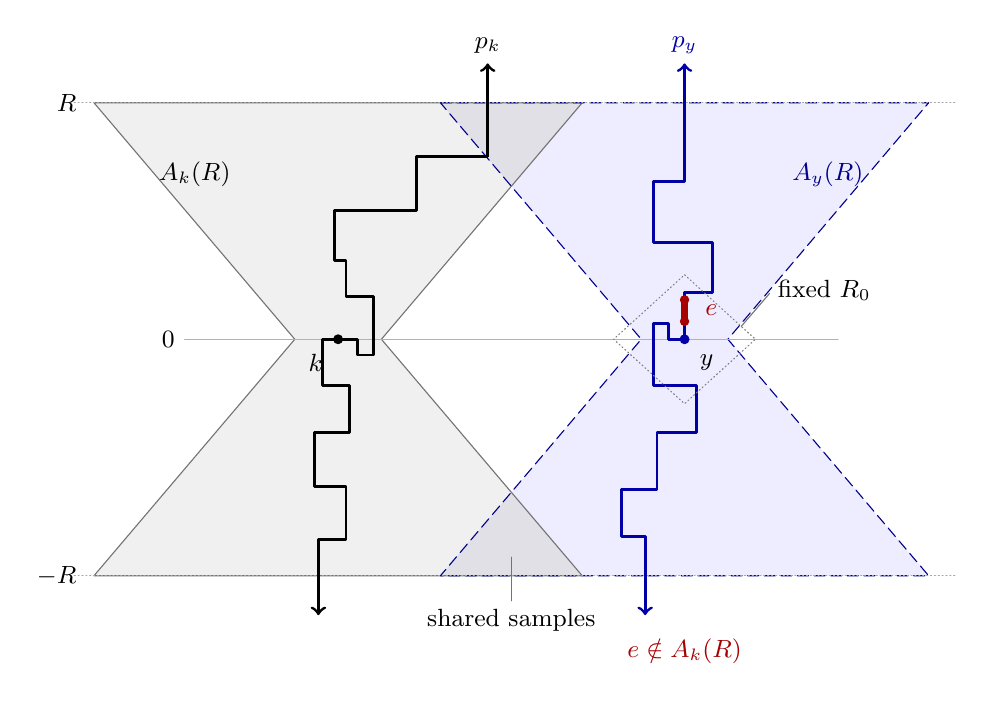
\begin{tikzpicture}[x=1cm,y=.91cm,font=\small,
  line cap=round,line join=round]
  \fill[black!6] (-5.3,3.3)--(.9,3.3)--(-1.65,0)
    --(.9,-3.3)--(-5.3,-3.3)--(-2.75,0)--cycle;
  \fill[blue!7!white] (-.9,3.3)--(5.3,3.3)--(2.75,0)
    --(5.3,-3.3)--(-.9,-3.3)--(1.65,0)--cycle;
  \fill[blue!18!black!12] (0,2.1353)--(.9,3.3)--(-.9,3.3)--cycle;
  \fill[blue!18!black!12] (0,-2.1353)--(.9,-3.3)--(-.9,-3.3)--cycle;
  \draw[black!55] (-5.3,3.3)--(.9,3.3)--(-1.65,0)
    --(.9,-3.3)--(-5.3,-3.3)--(-2.75,0)--cycle;
  \draw[blue!55!black,dash pattern=on 4pt off 2pt]
    (-.9,3.3)--(5.3,3.3)--(2.75,0)
    --(5.3,-3.3)--(-.9,-3.3)--(1.65,0)--cycle;
  \draw[black!35,densely dotted] (-5.65,3.3)--(5.65,3.3);
  \draw[black!35,densely dotted] (-5.65,-3.3)--(5.65,-3.3);
  \draw[black!30] (-4.15,0)--(4.15,0);
  \node[left] at (-5.4,3.3) {$R$};
  \node[left] at (-5.4,-3.3) {$-R$};
  \node[left] at (-4.15,0) {$0$};
  \node at (-4.02,2.3) {$A_k(R)$};
  \node[text=blue!55!black] at (4.02,2.3) {$A_y(R)$};

  \draw[line width=1.05pt,->]
    (-2.2,0)--(-1.95,0)--(-1.95,-.22)--(-1.75,-.22)
    --(-1.75,.6)--(-2.1,.6)--(-2.1,1.1)--(-2.25,1.1)
    --(-2.25,1.8)--(-1.2,1.8)--(-1.2,2.55)--(-.3,2.55)
    --(-.3,3.85);
  \draw[line width=1.05pt,->]
    (-2.2,0)--(-2.4,0)--(-2.4,-.65)--(-2.05,-.65)
    --(-2.05,-1.3)--(-2.5,-1.3)--(-2.5,-2.05)
    --(-2.1,-2.05)--(-2.1,-2.8)--(-2.45,-2.8)--(-2.45,-3.85);
  \draw[blue!65!black,line width=1.05pt,->]
    (2.2,0)--(2.2,.65)--(2.55,.65)--(2.55,1.35)
    --(1.8,1.35)--(1.8,2.2)--(2.2,2.2)--(2.2,3.85);
  \draw[blue!65!black,line width=1.05pt,->]
    (2.2,0)--(2,0)--(2,.22)--(1.8,.22)--(1.8,-.65)
    --(2.35,-.65)--(2.35,-1.3)--(1.85,-1.3)
    --(1.85,-2.1)--(1.4,-2.1)--(1.4,-2.75)
    --(1.7,-2.75)--(1.7,-3.85);
  \node[above] at (-.3,3.85) {$p_k$};
  \node[above,text=blue!65!black] at (2.2,3.85) {$p_y$};
  \fill (-2.2,0) circle (1.8pt);
  \fill[blue!65!black] (2.2,0) circle (1.8pt);
  \node[below left=2pt] at (-2.2,0) {$k$};
  \node[below right=2pt] at (2.2,0) {$y$};

  \draw[black!50,densely dotted] (2.2,.9)--(3.1,0)
    --(2.2,-.9)--(1.3,0)--cycle;
  \draw[red!65!black,line width=2.5pt] (2.2,.25)--(2.2,.55);
  \fill[red!65!black] (2.2,.25) circle (1.7pt)
    (2.2,.55) circle (1.7pt);
  \node[right=4pt,text=red!65!black] at (2.2,.4) {$e$};
  \draw[black!55] (3.28,.64)--(2.92,.18);
  \node[anchor=west] at (3.26,.68) {fixed $R_0$};
  \draw[black!55] (0,-3.65)--(0,-3.04);
  \node at (0,-3.92) {shared samples};
  \node[text=red!65!black] at (2.2,-4.35) {$e\notin A_k(R)$};
\end{tikzpicture}
\caption{Schematic envelopes of the truncated edge regions $A_k(R)$
and $A_y(R)$, not their exact lattice footprints. Overlap uses the same
raised sample for each edge, with no repeated increase. Every marked-path
edge in the slab belongs to its own region, so the union preserves both
paths' weights and geodesic property. The strictly raised edge $e$ lies
among the first $R_0$ steps from $y$ and outside $A_k(R)$ at sufficiently
large fixed separation. The near radius $R_0$ and this separation remain
fixed as $R$ grows.}
\label{fig:union}
\end{figure}

\newpage

\begin{proposition}[No repeated marked label]\label{prop:distinct-marks}
Almost surely, for each positive integer $M$, the selected upper labels
at distinct marked sites of $\Lambda$ are distinct.
\end{proposition}

\begin{proof}
Work on the common event specified above.  Suppose two marked sites
$k\ne y$ have $\rho_k=\rho_y$.  By \Cref{lem:union} both selected
bigeodesics persist with this label in $T^*=T^{k,y,R}$, where $R=R(M)$.
By \Cref{cor:same-busemann} their upper and lower Busemann functions in
this metric agree; denote the common pair by $B^+,B^-$.  For a vertex
$u$ on $p_y$, the bigeodesic inequality of \Cref{lem:opposite}, based
first at $k$ on $p_k$ and then at $u$ on $p_y$, gives
\[
 B^+(k,u)+B^-(k,u)\leq0,\qquad
 B^+(u,k)+B^-(u,k)\leq0.
\]
Additivity and antisymmetry therefore imply
\begin{equation}\label{eq:equal-sum-increments}
 B^+(k,u)+B^-(k,u)=0\qquad(u\in p_y).
\end{equation}

Take a raised edge $e=\{u,v\}$ among the first $R_0$ upper-arm edges of
$p_y$, and orient it toward the upper end, from $u$ to $v$.  Write $t_e^*$
for its weight in the union.  Calibration along the bigeodesic gives
\begin{equation}\label{eq:near-edge-calibration}
 B^+(u,v)=T^*(u,v)=t_e^*.
\end{equation}
Here the last equality holds because the one-edge segment of $p_y$
is itself minimizing.

Let $x_N^-,x_N^+$ tend respectively to the lower and upper ends of
$p_k$, with $k$ between them.  Set
\[
 L_N^*=T^*(x_N^-,u)+t_e^*+T^*(v,x_N^+),\qquad
 D_N^*=T^*(x_N^-,x_N^+).
\]
This $L_N^*$ is the cost of an admissible finite walk, so
$L_N^*\geq D_N^*$.  As $p_k$ is a bigeodesic,
$D_N^*=T^*(x_N^-,k)+T^*(k,x_N^+)$.  The signs in the Busemann definition
then give, separately,
\begin{align*}
 T^*(x_N^-,u)-T^*(x_N^-,k)&\longrightarrow-B^-(k,u),\\
 T^*(v,x_N^+)-T^*(k,x_N^+)&\longrightarrow-B^+(k,v).
\end{align*}
It follows that
\begin{align}
 L_N^*-D_N^*
 &\longrightarrow -B^-(k,u)-B^+(k,v)+t_e^*\notag\\
 &=-\bigl[B^-(k,u)+B^+(k,u)\bigr]-B^+(u,v)+t_e^*=0,
 \label{eq:detour-excess}
\end{align}
by \eqref{eq:equal-sum-increments} and \eqref{eq:near-edge-calibration}.

Choose minimizing finite approach paths in $T^*$ from $x_N^-$ to $u$
and from $v$ to $x_N^+$, and join them by the specified traversal
$u\to v$ of $e$.  Call this finite walk $W_N$.  The approach paths
may intersect each other, the selected bigeodesics, or $e$ itself;
its cost is $L_N^*$ with every traversal counted.
By \Cref{lem:union}, the weight of $e$ in $T^{k,R}$ is its base weight
$X_e$.  Thus
\[
 \Delta=t_e^*-X_e\geq g>0.
\]
On returning from $T^*$ to $T^{k,R}$ every traversal weakly decreases
in cost, and the named middle traversal decreases by $\Delta$.
Consequently
\begin{equation}\label{eq:walk-saving}
 \operatorname{cost}_{T^{k,R}}(W_N)\leq L_N^*-\Delta.
\end{equation}
Any further traversal of the same edge can only increase this saving.
On the other hand, the segment of $p_k$ between $x_N^-$ and $x_N^+$
has cost $D_N^*$ in both metrics, again by \Cref{lem:union}.
For sufficiently large finite $N$, \eqref{eq:detour-excess} gives
$L_N^*-D_N^*<\Delta$.  Then \eqref{eq:walk-saving} makes $W_N$ strictly cheaper in
$T^{k,R}$ than that segment, a contradiction.  This is a pathwise
argument for every marked pair on the common event, and hence proves
the assertion simultaneously for the countably many $M$.
\end{proof}
